\chapter{データ} 

\section{SDO / AIA}
モデルの学習及び評価データとして、NASAのSolar Dynamic Observatory(SDO)\cite{pesnell2012solar}のAtmospheric Imaging Assembly(AIA)\cite{lemen2012atmospheric}で撮影された紫外線観測データを用いた。

SDOはNASAのLiving With a Star(LWS)プログラムの一つとして2010年2月に打ち上げられた太陽観測衛星である。
AIA、Helioseismic and Magnetic Imager(HMI)、Extreme Ultraviolet Variability Experiment(EVE)などの高い空間解像度、時間分解能を持つ観測機器を搭載している。
その観測データを用いることにより、太陽物理学、宇宙天気、また地球環境に関する理解や洞察を深めることが期待されている。
AIAは主に太陽大気を観測する観測機器であり、4つの望遠鏡で構成されている。
4096×4096、約1.5秒角の空間解像度をもち、12秒ごとに太陽全球の画像を観測している。
また、7つの極紫外線フィルターと、2つの紫外線フィルター、および1つの可視光フィルターを持ち、広範な温度帯で太陽大気を観察することを可能にしている。

これらのデータはJoint Science Operations Center(JSOC) によって提供されており、Pythonの太陽物理学を支援するライブラリであるSunpyを用いてダウンロードすることができる。


\subsection{AIA 211Å}
観測されるイオン、温度範囲、主な観測対象(活動領域、CHなど)

\subsection{AIA 193Å}
\subsection{AIA 171Å}

\begin{figure}[h]
    \centering
    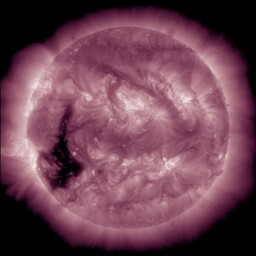
\includegraphics[width=0.8\textwidth]{figures/latest_256_0211.jpg}
    \caption{SDO/AIAの211Åフィルターで撮影された太陽全球紫外線像。強調のために紫色に色付けされている。球面の中上部から中下部には明るく輝く活動領域が見られ、左下部に暗くコロナホールが観測できる。}
    \label{fig:sample_aia211}
\end{figure}
\section{前処理}


本研究で用いるデータセットには、SDO/AIA望遠鏡のデータが提供されている2010年5月から、2022年10月までのデータが含まれている。\\
この期間に存在するデータから、4時間ごとにデータを抽出し、各波長ごとに約22000枚(正確な方がいい?)をデータセットに含んでいる。これらのデータを、24枚の画像を1セットとして分割する。各セットは24枚の時系列に並んだ画像で構成され、太陽の時間的依存性および空間的情報を同時に捉えている。24枚のうち、前半の12枚、すなわち44時間後までを入力データ、後半の12枚、すなわち48時間後から92時間後までを出力データとして扱う。学習の際は、前半の12枚に対して後半の12枚を教師データとして扱い、テストの際は12枚の画像データに続くモデルにとって未知の12枚を再現できるか検証する。


このデータセットは第24太陽活動周期の初期から、第25周期の初期までの観測データを網羅している。この時間範囲には、太陽活動の活発性が高いフェーズと低いフェーズの両方が含まれている。従って、このデータセットは太陽活動の活発性に依存しない可能性が高く、その汎化能力に対する期待が一定程度裏付けられる。



\begin{table}[h]
    \centering
    \begin{tabular}{|c|c|c|}
    \hline
    実験 & 実験1 & 実験2 \\
    \hline\hline
    入力波長 & 211Å & 171Å,193Å,211Å \\
    \hline
    出力波長 & \multicolumn{2}{c|}{211Å} \\
    \hline
    総枚数 & 22000 & 66000 \\
    \hline
    セット数 & \multicolumn{2}{c|}{232} \\
    \hline
    セットごとの枚数 & \multicolumn{2}{c|}{入力12 → 出力12} \\
    \hline
    解像度 & \multicolumn{2}{c|}{512 * 512} \\
    \hline
    \end{tabular}
    \caption{各実験でのデータセット}
    \label{tab:my_label}
\end{table}

\subsection{不正な画像の除去}
SDO/AIA望遠鏡で撮影された全球画像には、露光時間が他の画像より極端に低い、画像内に太陽全体を捉えていない、などの不正な画像が含まれている。
確認することができた主な不正な画像を図\ref{fig:bad_aia_samples}に示す。

\begin{figure}[htbp]
    \centering
    \begin{subfigure}[b]{0.48\textwidth}
        
\includegraphics[width=\textwidth]{figures/bad_sample0.png}
        \caption{短い露光時間により、極端に暗い画像。}
    \end {subfigure}
    \hfill
    \begin{subfigure}[b]{0.48\textwidth}
        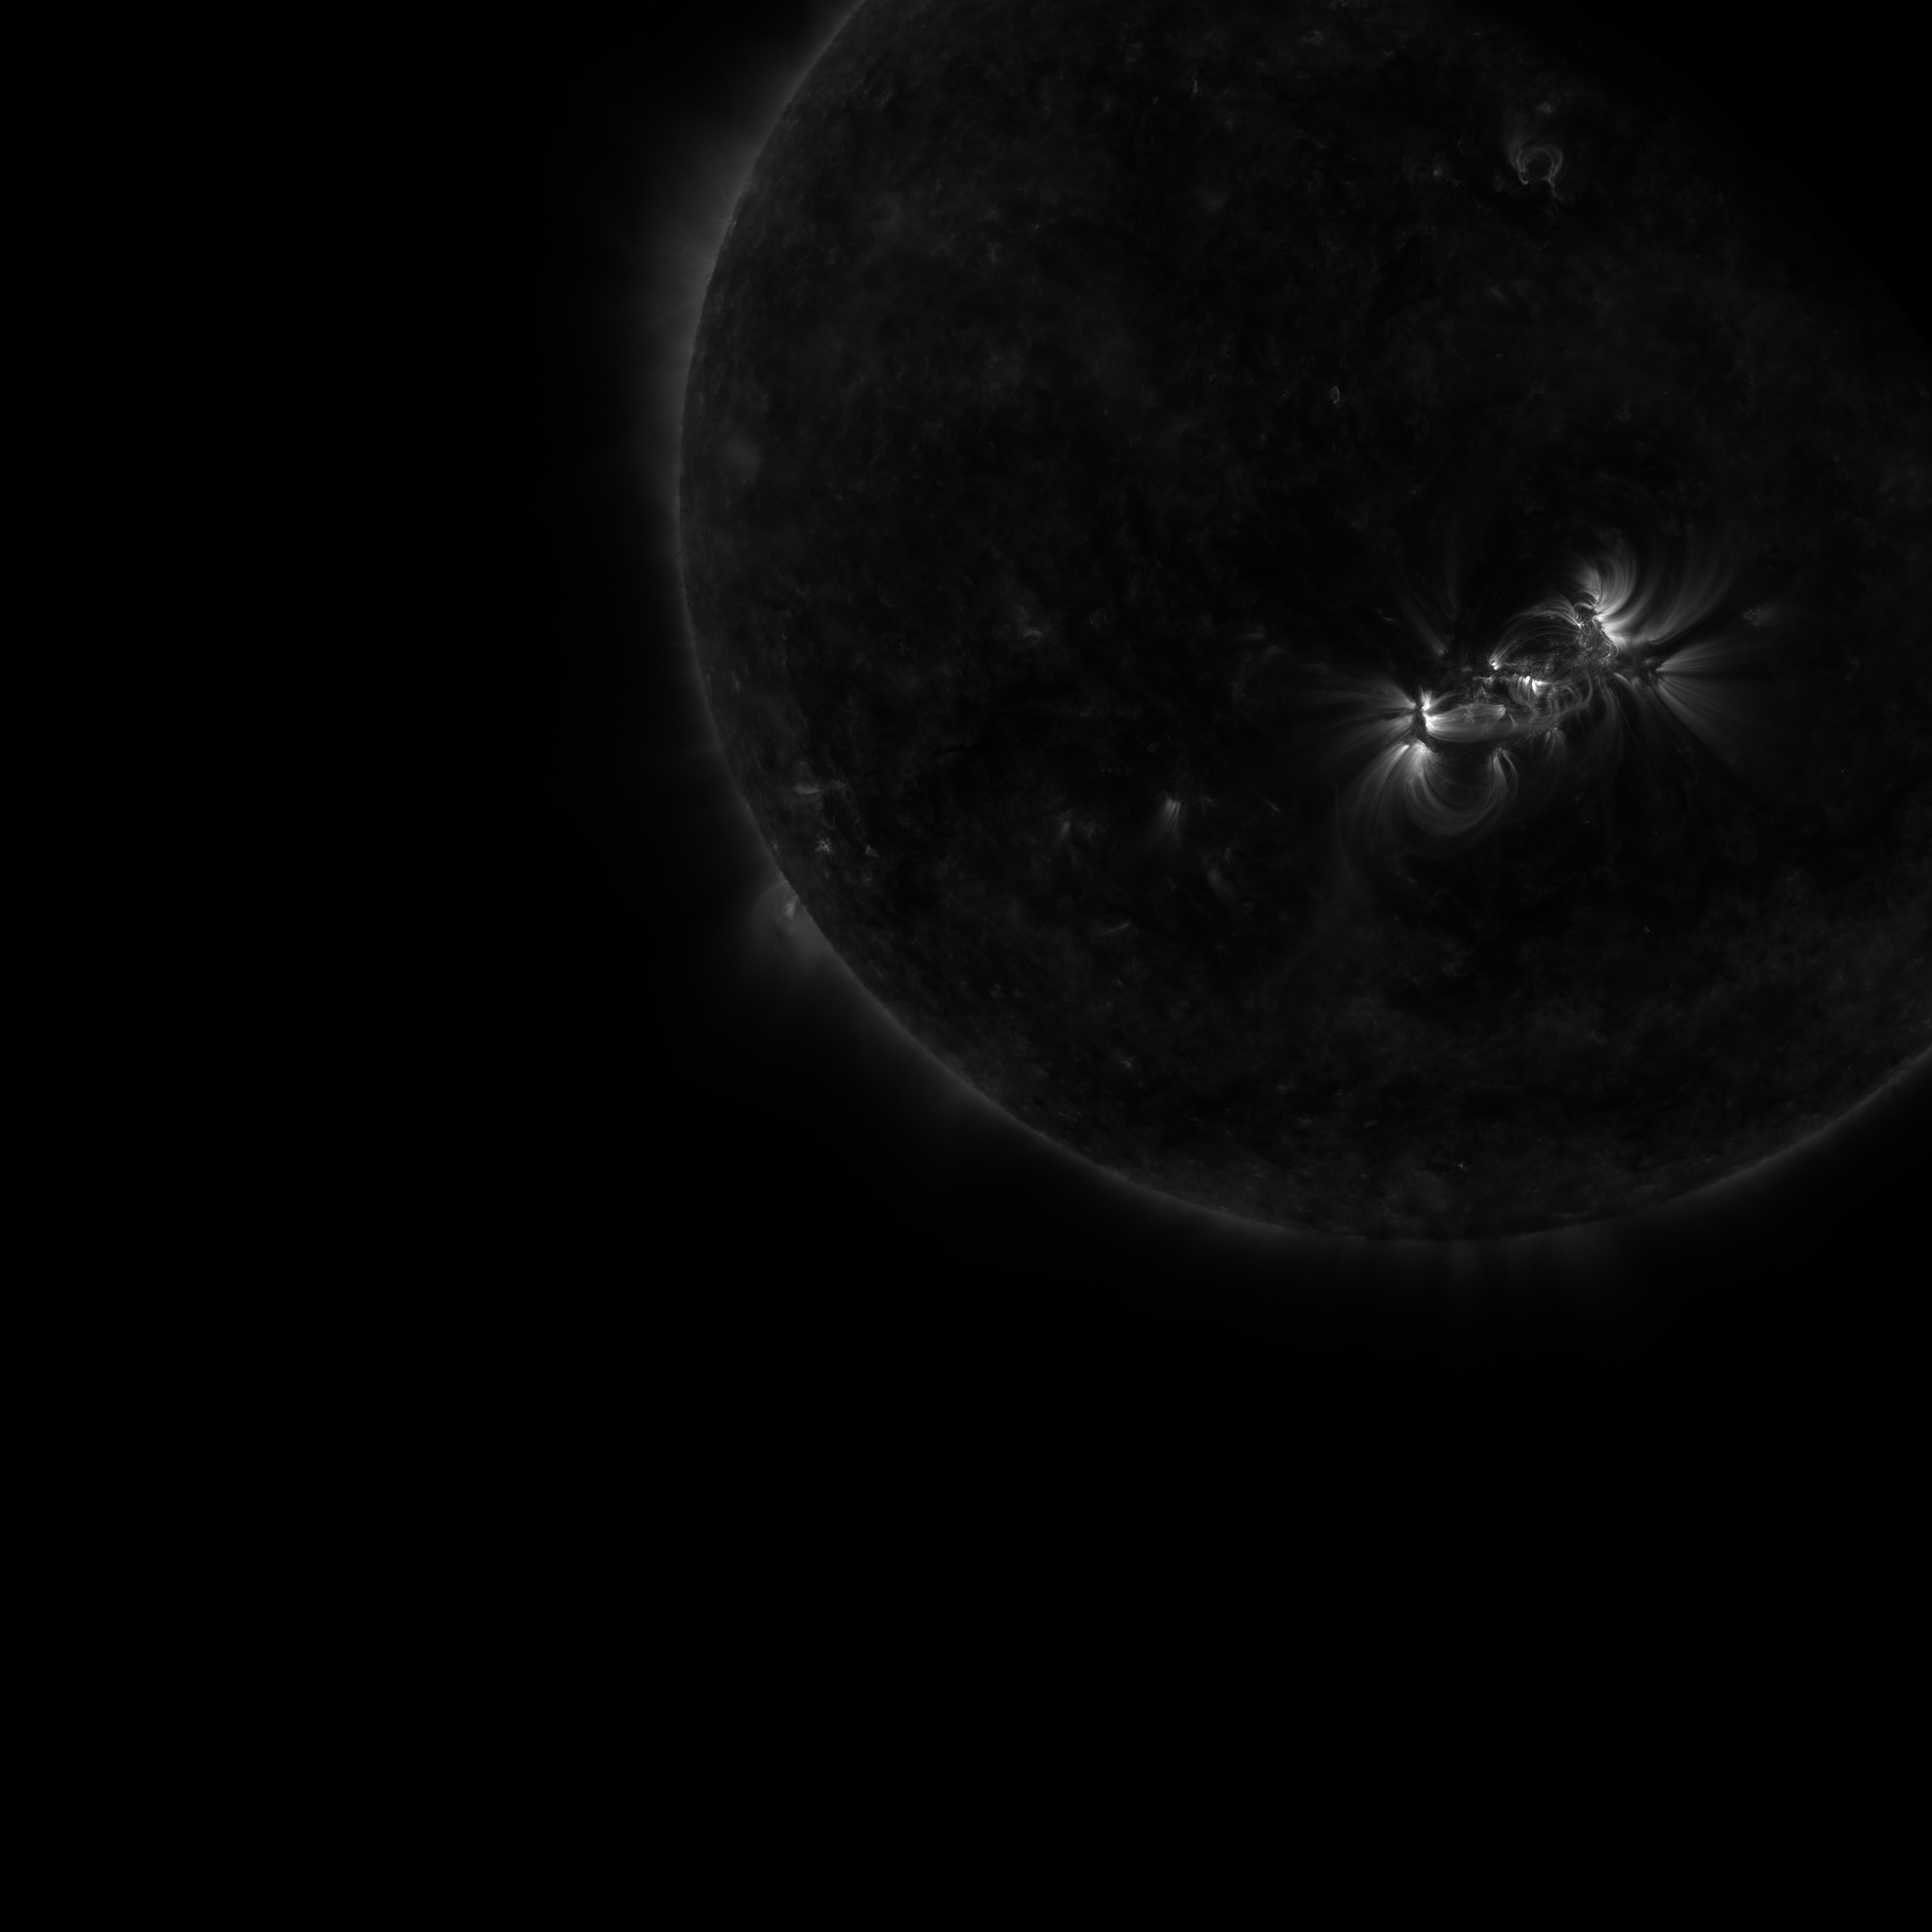
\includegraphics[width=\textwidth]{figures/bad_sample1.png}
        \caption{太陽が画像の中心にない画像。}
    \end {subfigure}
    \begin{subfigure}[b]{0.48\textwidth}
        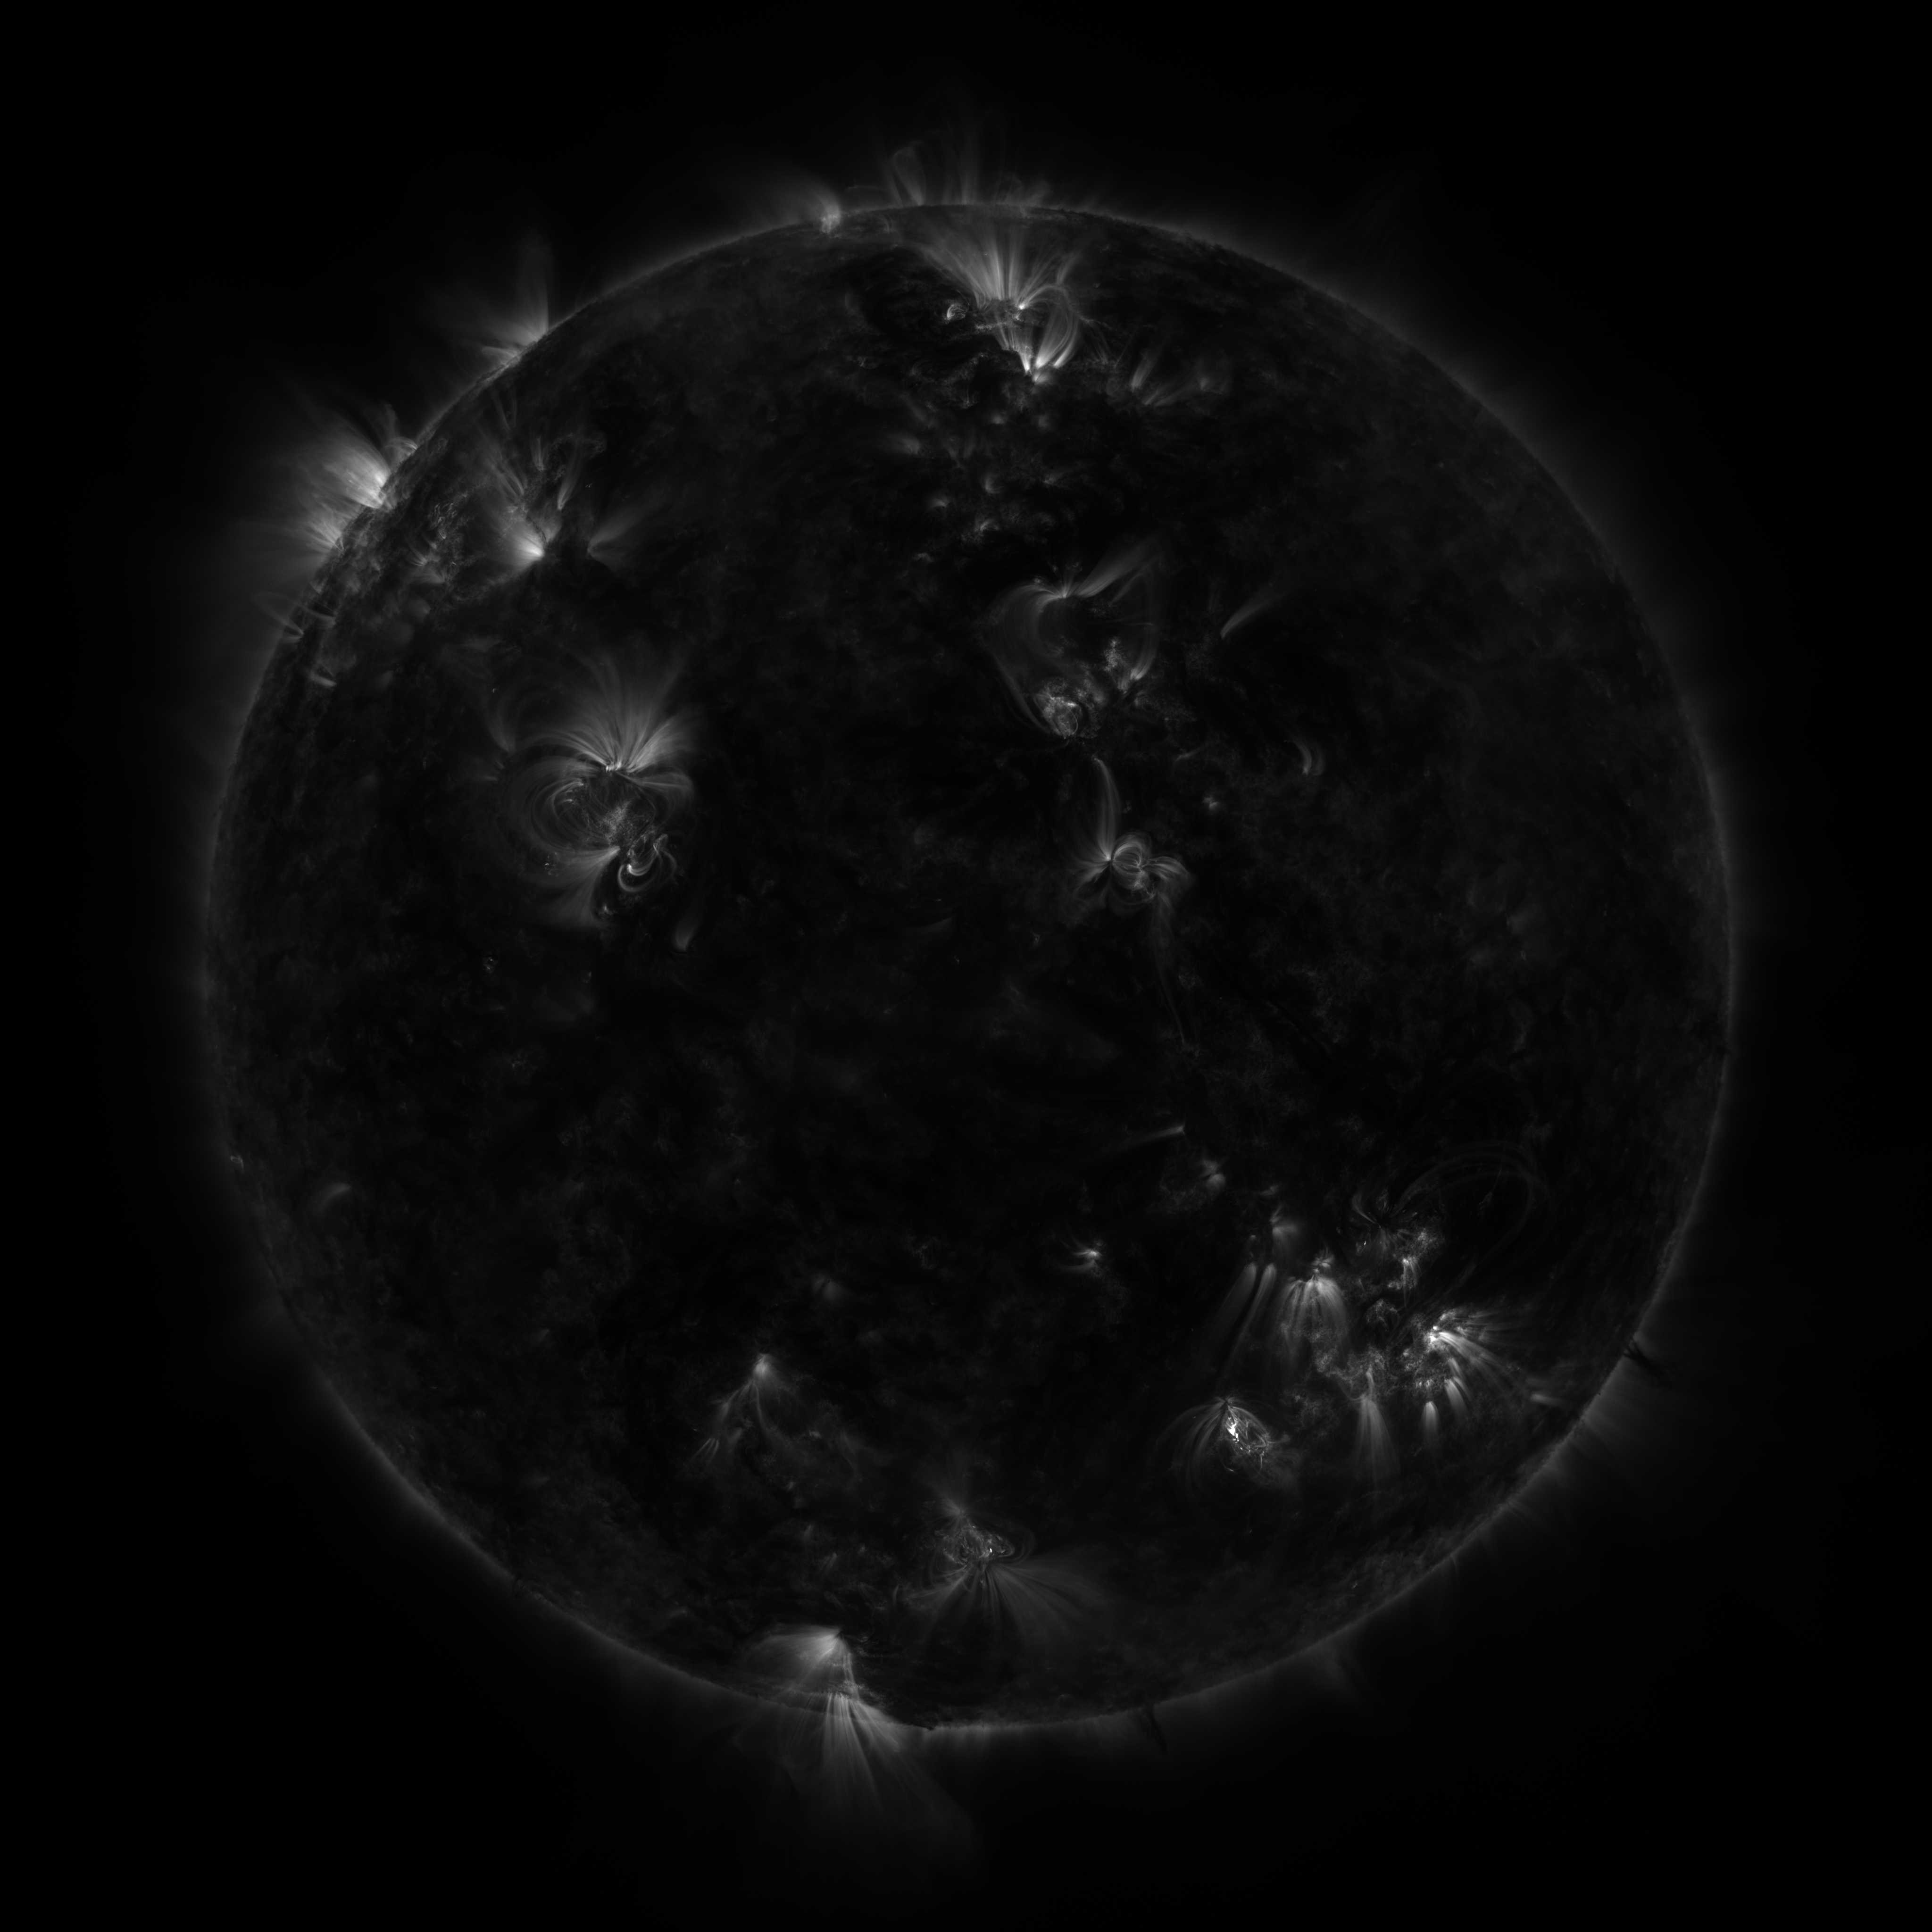
\includegraphics[width=\textwidth]{figures/bad_sample2.png}
        \caption{衛星が回転しており、正しい角度で太陽が撮影されていない画像。活動領域の少ない左下部と右上部が極である。}
    \end {subfigure}
    \hfill
    \begin{subfigure}[b]{0.48\textwidth}
        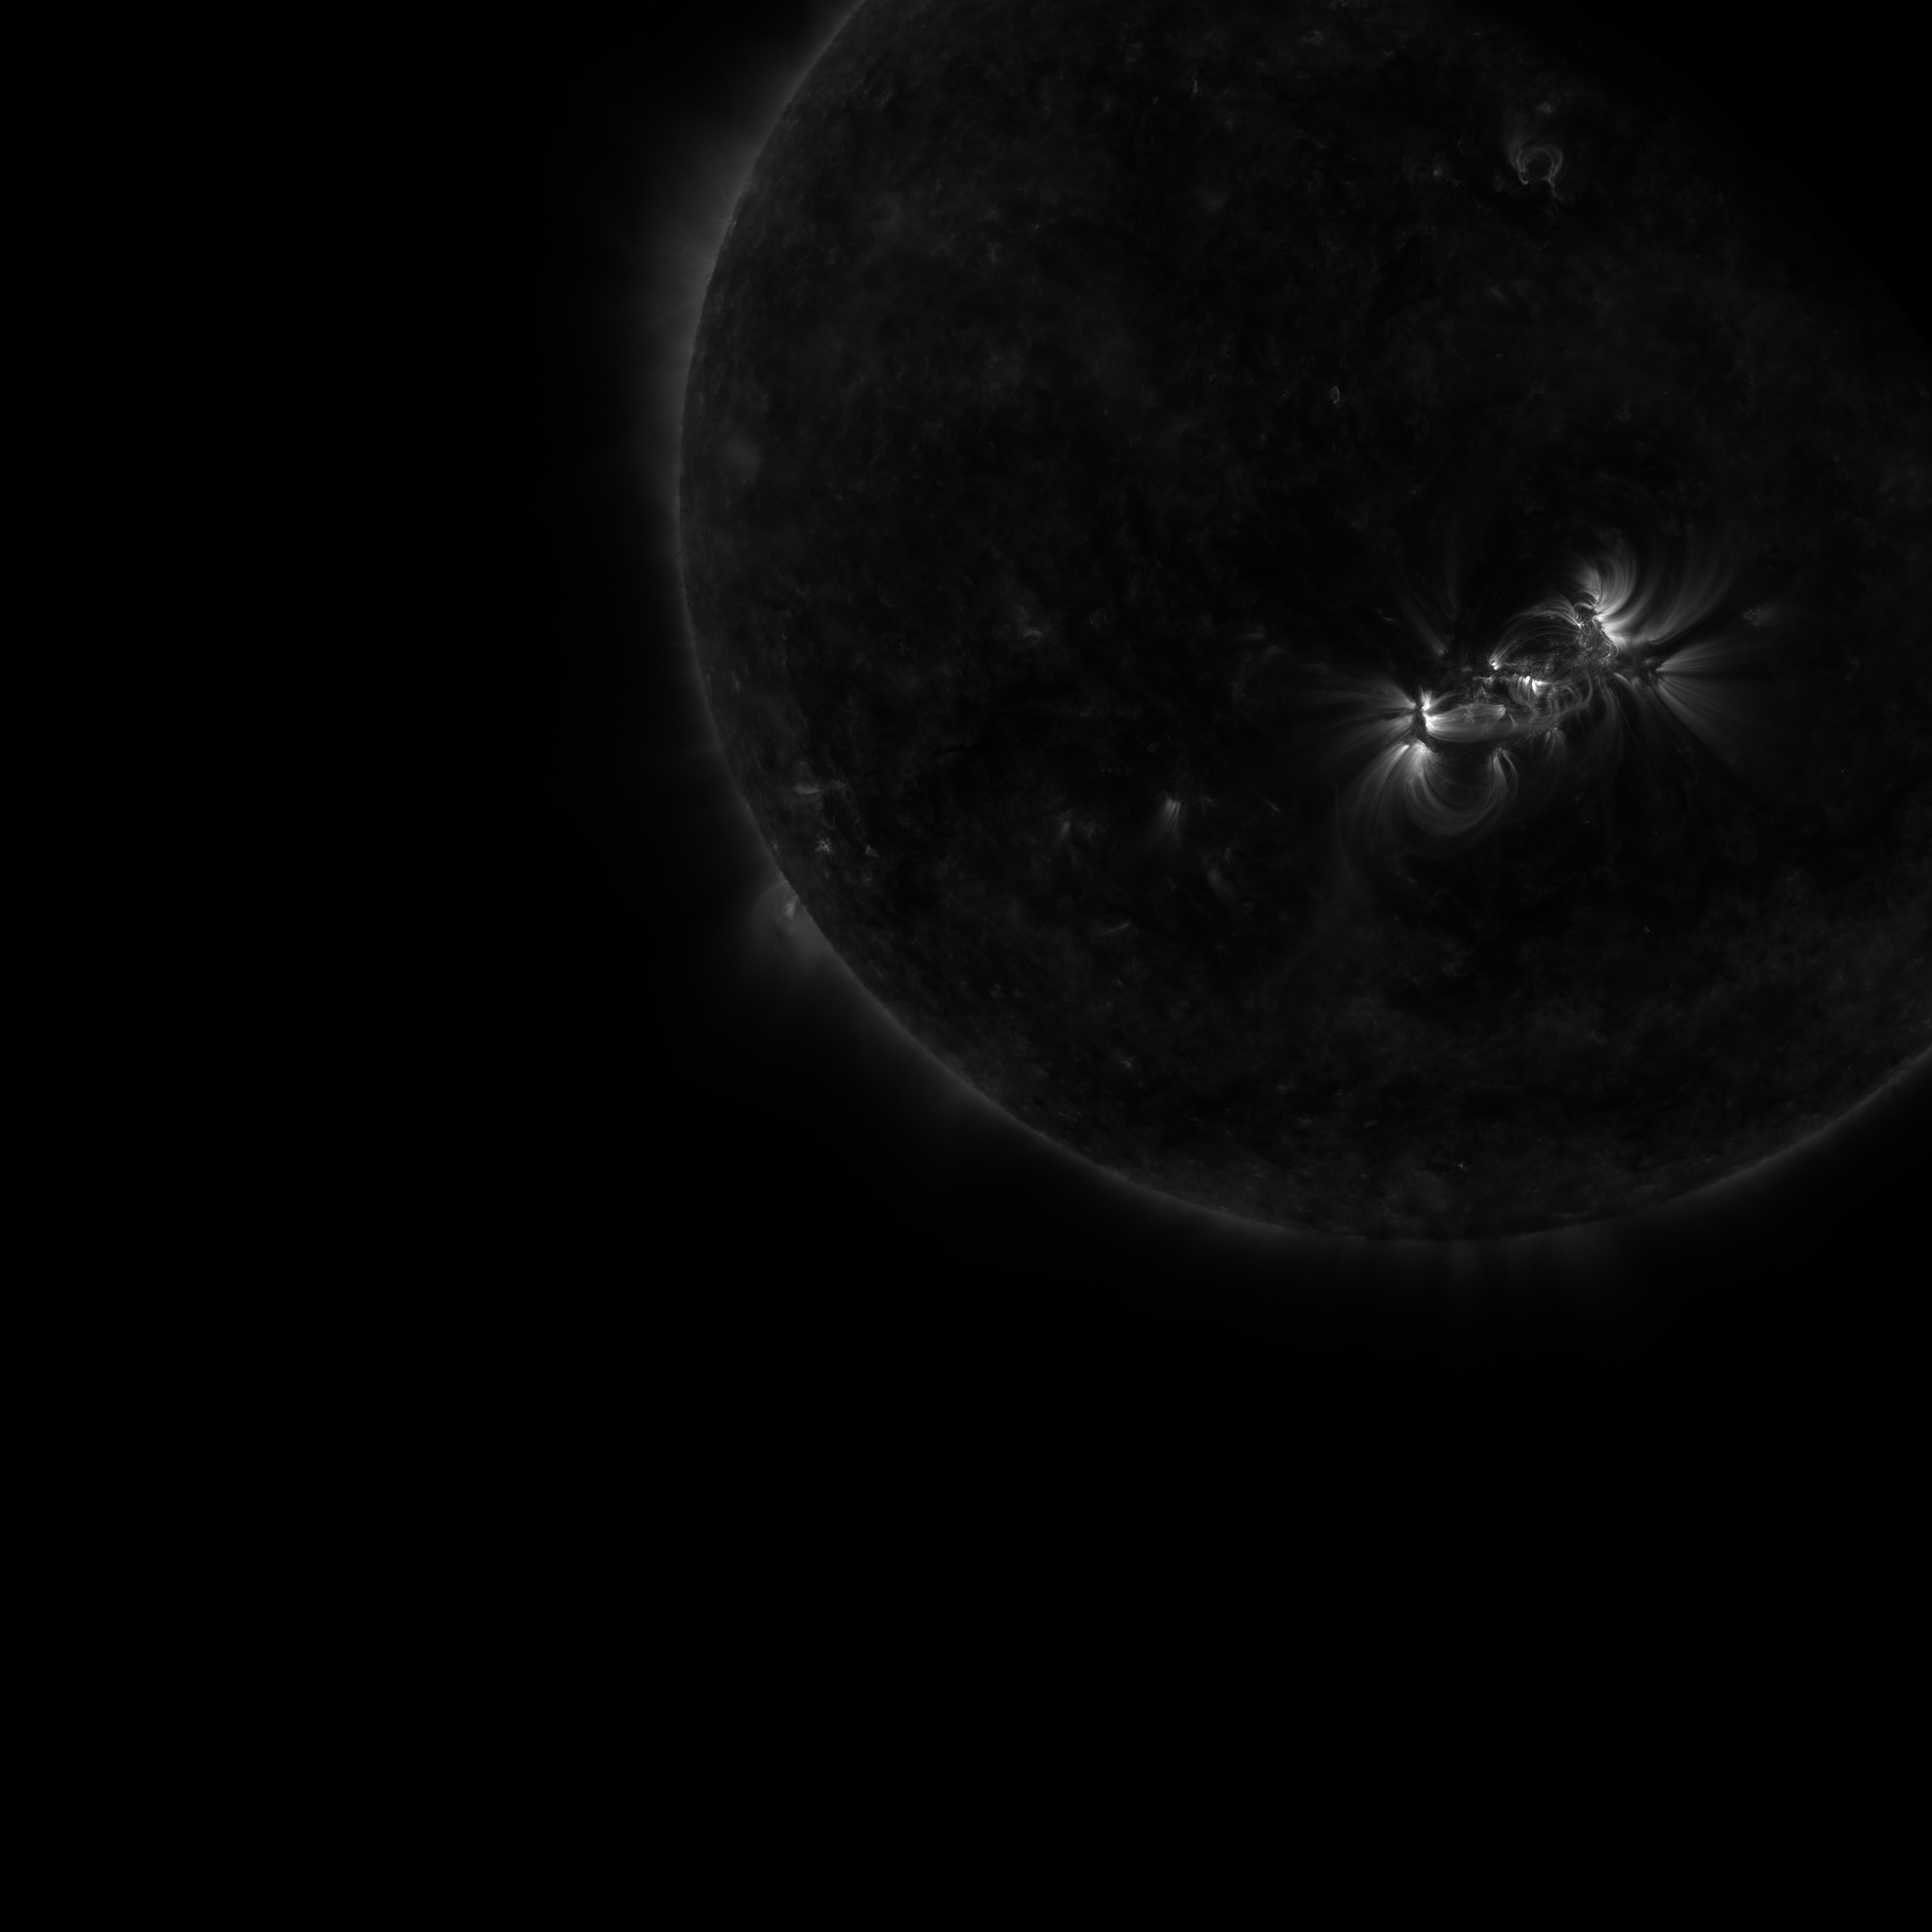
\includegraphics[width=\textwidth]{figures/bad_sample1.png}
        \caption{日蝕により太陽が隠されている画像}
    \end {subfigure}
    \caption{SDO/AIAにより観測された不正な画像の例}
    \label{fig:bad_aia_samples}
\end{figure}

これらの画像は、モデルの学習に悪影響を及ぼす可能性があるため、データセットから除去した。
機械学習のタスクによっては、十分なデータセットがあれば、モデルが不正な画像に対する頑健性を獲得し、不正な画像がデータセットに含まれていても、学習結果にあまり大きな影響を与えない場合がある。
しかし、本研究で行う動画予測は、データセットに含まれる画像がそのまま教師データとなるため、不正な画像は損失関数の計算、またはモデルの評価に大きな影響を与えるため、慎重に除去する必要がある。
データの除去には、FITSファイルのヘッダーに記録された各キーワードの値に対して閾値を設定して判定したのち、numpyによる輪郭検出を用いた月蝕判定関数により不正な画像を排除した。この流れを図に示す。
月蝕判定関数は、〜〜〜〜〜

\subsection{スケーリングと正規化}

\subsection{データセットの分割}

このようにして作成されたデータセットは、約1000セットになり、これを学習用データセットに約800セット、検証データセットに50セット,テストデータセットに50セットというように分割した。


